\documentclass[11pt, a5paper, parskip=half-, DIV=12]{scrartcl}

\usepackage{../endeavour}
\usepackage{../endeavour_book}

\version{0.1}

\begin{document}
% Colour Cover
\thispagestyle{plain}
\AddToShipoutPictureBG{
\begin{tikzpicture}[remember picture, overlay]
	\node () at (current page.center) {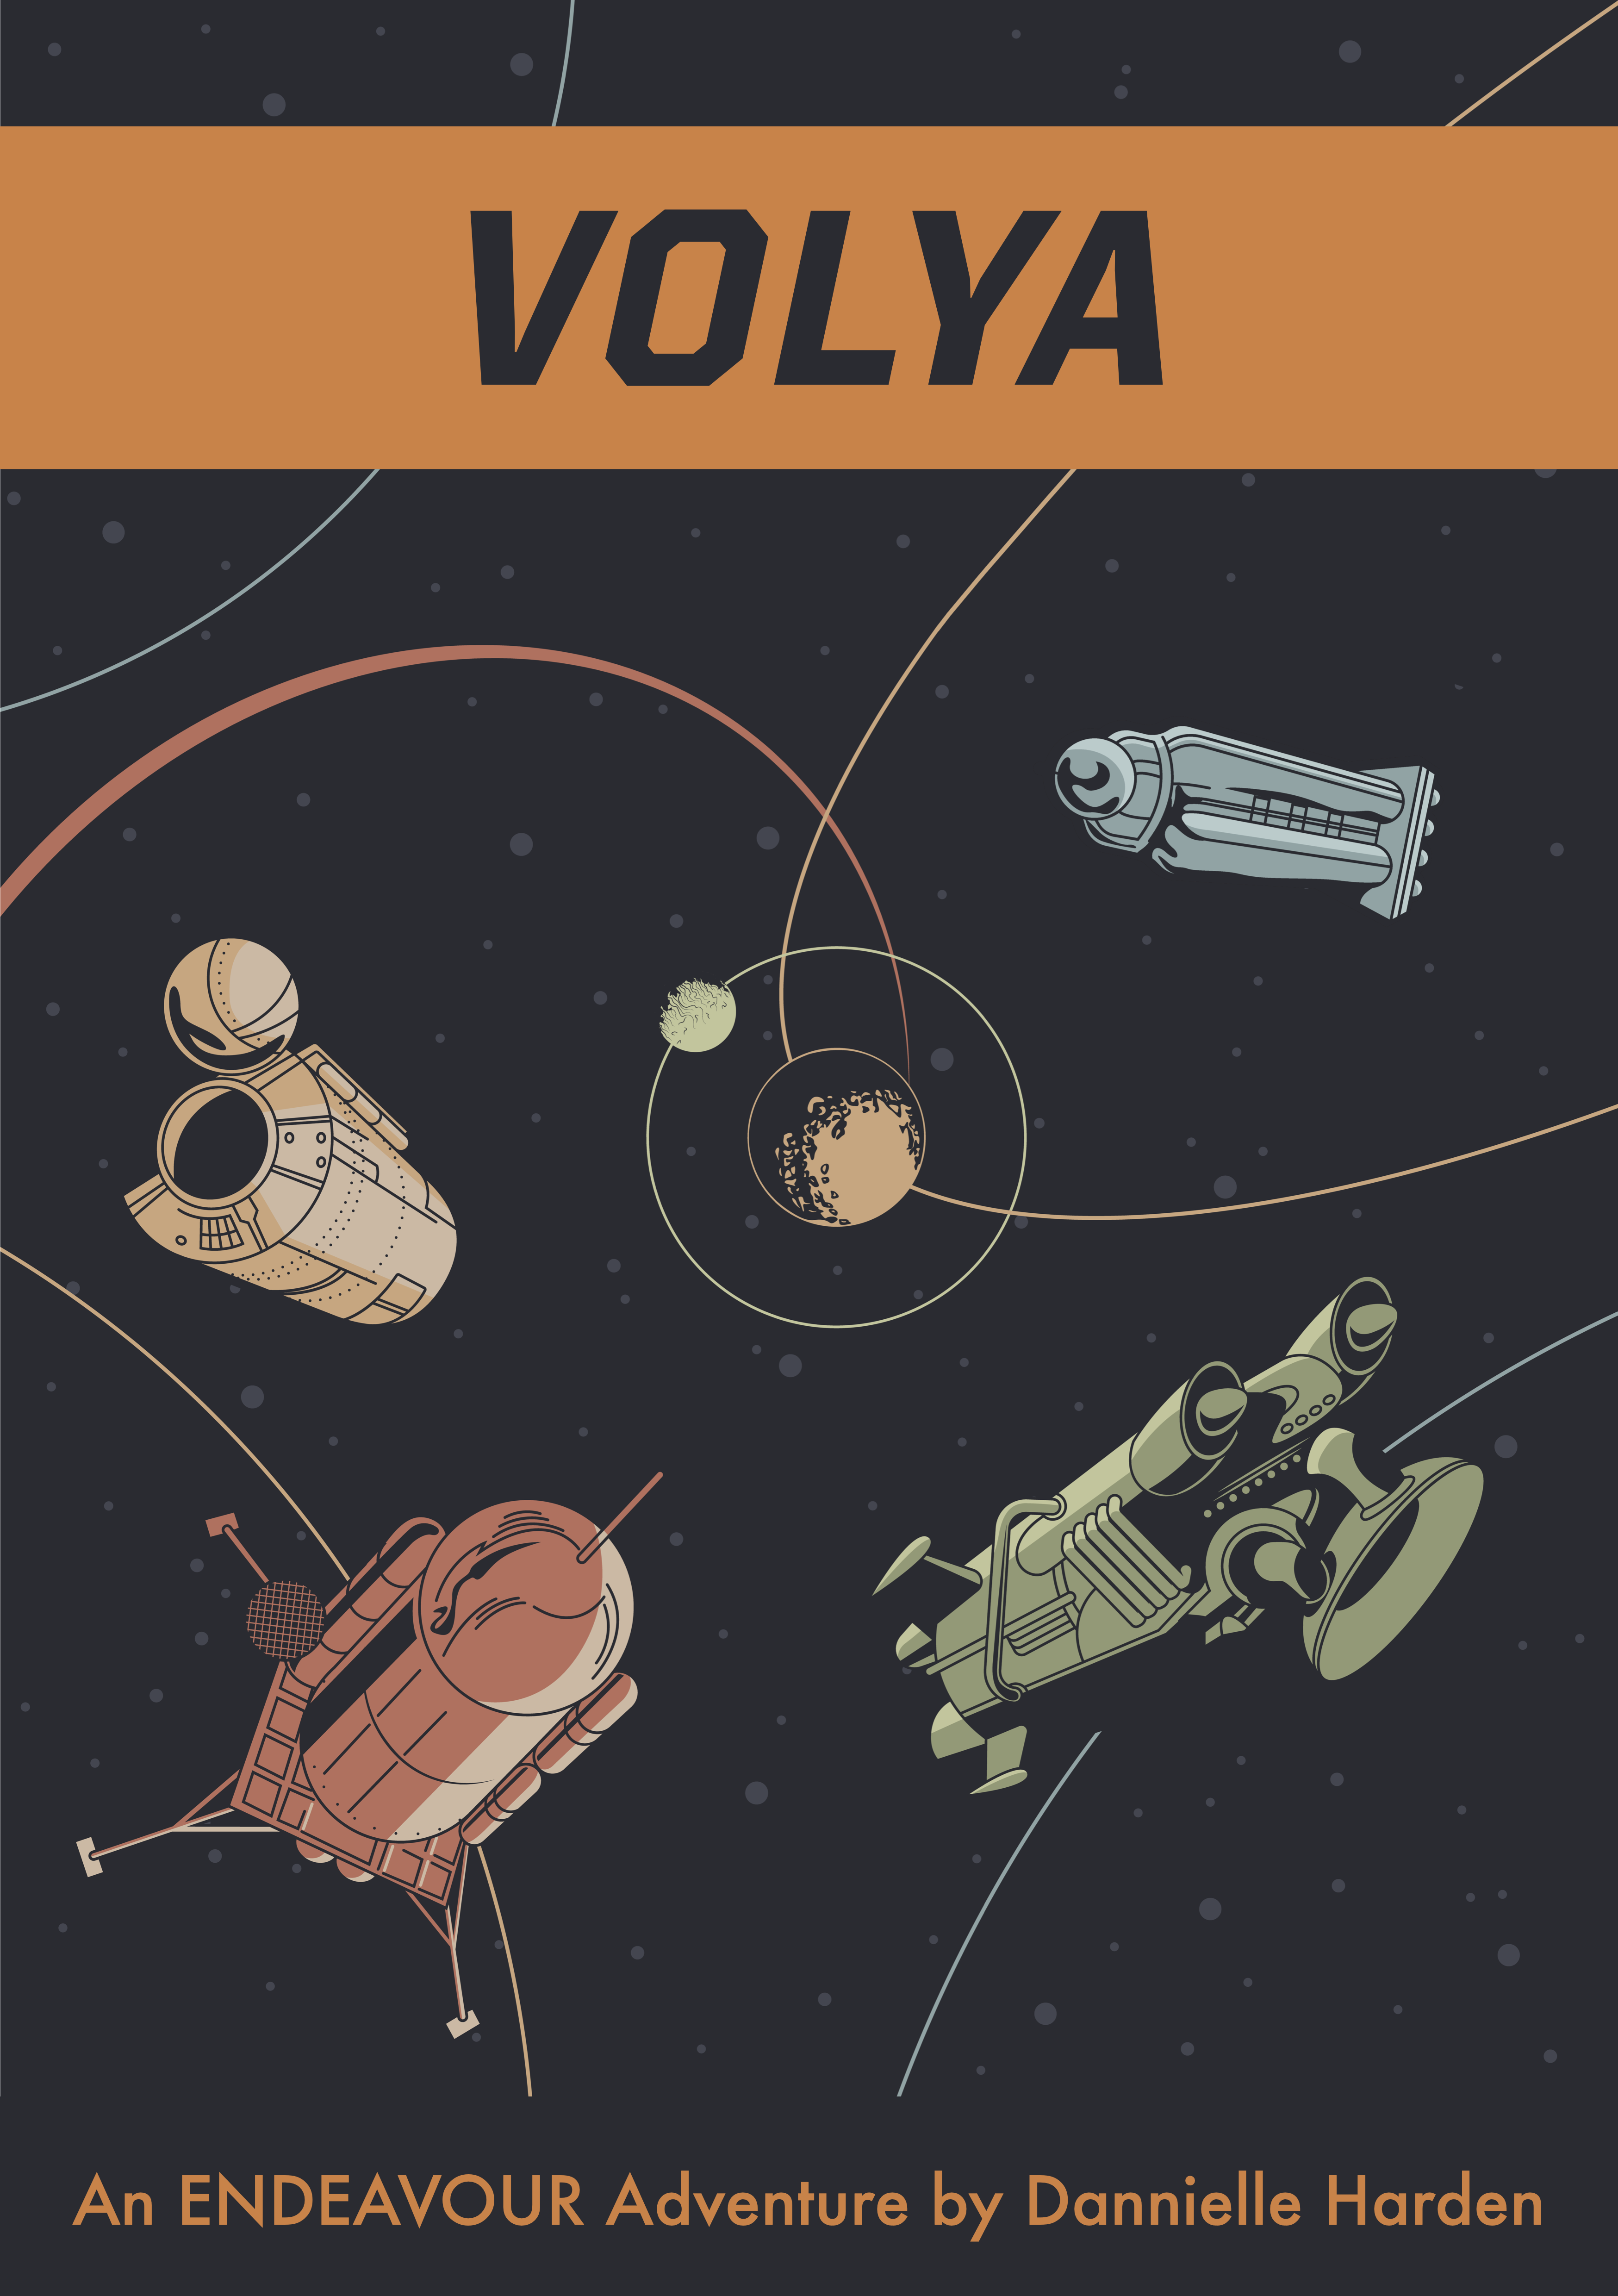
\includegraphics[width=\pagewidth, height=\pageheight]{Images/volya_cover.png}};
\end{tikzpicture}
}
{
\colorlet{headfootcolor}{LCARS_ORANGE}
\phantom{a}

\newpage
}

\ClearShipoutPicture
\AddToShipoutPictureBG{
	\begin{tikzpicture}[remember picture, overlay]
	\pic () at (current page.center) {starfield};
		\node[endeavour_box, minimum width=12.6cm, minimum height=18.8 cm] at (current page.center) {};
	\end{tikzpicture}
}

\setcounter{page}{1}
\setmainfont{TeX Gyre Schola}
\normalsize
\raggedright

\section*{Volya}
\textit{\textbf{Captain's Log:} Three weeks ago, the government of Volya reported a dramatic surge in both petty crime and in missing person cases. Since that time, however, the ICF been unable to contact the Volyans to determine the full extent of the problem. We have been dispatched to the planet to investigate further.}

%\textit{Volya is renowned for having a strict society with complex cultural norms. As such, we have undergone specialized training while en route to acquire a basic understanding of Volyan etiquette. Furthermore, the landing party have been issued special uniforms which shroud the entire body from view; standard-issue ICF uniforms would be considered lewd.}

\textit{Volya has a strict society with complex cultural norms. As such, we have undergone specialized training in Volyan etiquette while en route. Furthermore, we have been issued special uniforms which shroud the entire body from view; standard-issue ICF uniforms would be considered lewd.}

%\textit{On a personal note, the last week of training has been exhausting. In that time, I apparently discovered several hundred new ways to give offense.  I can only hope the landing party have fared better in their studies.}

\subsection*{Arrival}
As you approach Volya, you find many cargo ships in orbit.
The traffic congestion around the planet is beginning to pose a serious safety threat. The density of ships is such that any accidents would be likely to initiate a cascade of collisions.

%The traders hail you to report that they have been unable to contact anyone on the planet below.
The traders report that they have been unable to contact the Volyan authorities. 
%A few of the traders are Volyans who have have recently returned home. They have been unable to contact their families or business associates.
%One trader is a Volyan who has recently returned home.  He has been unable to contact anyone other than \textbf{Prash}, an antique dealer and long-time customer.
One Volyan trader has spoken with an old friend named \textbf{Prash}. The trader's daughter, \textbf{Diminin}, works for Prash, but has been missing for several weeks.

%The traffic congestion around Volya is beginning to pose a serious safety threat. The density of ships is such that any accidents would be likely to initiate a cascade of collisions. %The resulting debris field from such an ablation cascade would pose a serious threat to navigation for many years.
\subsubsection*{Duty of Care}
\begin{itemize}
	\item \textit{Will you try to establish order among the merchant ships?} \\ \textbf{Operations \& Engineering} vs. \textbf{Traffic Jam (2d8)}. \\ If you do not prevail at this challenge, then during the Crisis you must face the following \textbf{Threat:} A cascade of collisions makes travel to or from Volya impossible.  
	\item \textit{Or will you try to contact the Volyan government and begin your investigation without further delay?} \textbf{Leadership \& Negotiation} vs. \textbf{Volyan Etiquette}. If you prevail, gain a 1d6 Advantage die on all challenges vs. Volyan Etiquette.
\end{itemize}

\newpage

\subsection*{Trials}
\subsubsection*{Augmented Reality}
Zephan appears to be entirely vacant of people. Oddly, the facades of most buildings have been replaced with featureless white panels.
%As you walk around, however, you are occasionally buffeted as if by someone rudely pushing their way through a crowd.
%\textit{Can you discover why you can't see or hear anyone?} \textbf{Science \& Medicine} vs. \textbf{Visors (3d8)}.
Without Visors, the city is nearly impossible to navigate. \textit{Can you find a way to acquire a set of Visors?} \\ \textbf{Operations \& Engineering} vs. \textbf{Volyan Etiquette}.

\subsubsection*{Minding His Own Business}
Prash's shop is remarkable for being one of the few still displaying traditional decorations. Prash politely explains that he cannot treat with offworlders without his assistant, Diminin, present to observe.
%Sadly, she has been missing for several weeks.
He refuses to violate Diminin's privacy by saying more.
\textit{Can you convince Prash to tell you where you can find Diminin?} \textbf{Strategy \& Tactics} vs. \textbf{Prash}.

\subsubsection*{Missing Person}%Hikikomori
In contrast to the featurelessness of the city's public spaces, Diminin's home is a riot of vulgar (by Volyan standards) self-expression. She is reluctant to entertain visitors, and will not meet with you here. She has not left her home without a Visor since she acquired one several weeks ago. \textit{Can you help Diminin find a way to more confidently reengage with Volyan society?} \textbf{Science \& Medicine} vs. \textbf{Diminin}.

\subsection*{Crisis}

\begin{itemize}
	\item \textit{Will you try to disable/outlaw Visor technology?} \\ \textbf{Threats:} Volya withdraws from the ICF, citing violations of their sovereignty. Many Volyans who find traditional etiquette stifling withdraw completely from public life.
	\item \textit{Or will you try to help the Volyans find less disruptive ways to incorporate Visor technology into their society?} \\ \textbf{Threats:} Organized crime surges. A revolutionary counterculture develops among marginalized Volyans.   
\end{itemize}

\newpage

\subsection*{Characters}
\begin{description}
%	\item[Artem (d8):] Merchant (d8), Captain (d8), Practical (d8).
	%\\ \textbf{\textsc{Volyan}} (Volyan Etiquette applies to any Leadership \& Negotiations or Strategy \& Tactics challenges).
	\item[Prash (d8):] Antique Dealer (d8), Paternal (d8). \\ \textbf{\textsc{Traditional}} (Volyan Etiquette applies to any Leadership \& Negotiation or Strategy \& Tactics challenges).
	\item[Diminin (d6):] Clumsy (d6), Shy (d6), Ashamed (d6).
	\item[Volyan Etiquette (d10):] Greetings / Partings (d6), Honorifics (d8), Public Announcements (d10 \textit{Sensitive}).
\end{description}

\subsection*{Places}
\begin{description}
	\item[Zephan:] The capital city of Volya. It is a metropolis located in a desert near the terminator that separates the light and dark sides of the tidally-locked planet.
	\item[Marketplace:] A large building to shade trade goods from the sun. Once brightly patterned and ornately decorated, its facade is now a featureless blank canvas.
\end{description}

\subsection*{Mysteries}
\begin{description}
	\item[Personal cloaking was recently invented on Volya.] \phantom{} \\ The personal cloaking device is called a Visor. A Visor conceals its wearer from anyone whom they have not identified as a contact. Such permissions can be revoked at any time. \textit{Why would the Volyans want to hide from each other? What are the advantages / disadvantages of so severely limiting what information is publicly available?}
	\item[Volyans believe in a fundamental right to privacy.] \phantom{} \\ Volyan magistrates have ruled that the use of personal cloaking technology cannot be infringed upon in any way. Accordingly, Visor usage has quickly become ubiquitous. \textit{How has the free use of personal cloaking changed Volyan Society? How has it impacted security and public safety?}
\end{description}

\newpage

\section*{Acknowlegements}
Much of the look and feel of \ENDEAVOUR{} is derived from its art, all of which was created by \textbf{svekloid}. This art was assembled from multiple collections available online at \href{http://shutterstock.com}{shutterstock.com} and then modified by Michael Purcell.  

\subsection*{Playtesters} \label{subsection:playtesters}
The following people helped to create \ENDEAVOUR{} by playing early versions of the game and providing invaluable feedback.\vspace{-1.75ex}
\begin{multicols}{2}
\begin{itemize}[noitemsep]
  \item Keydan Bruce
  \item Dannielle Harden
  \item Andrew Hellyer
%  \item Sarah Hewat
%  \item Scott Joblin
%  \item Sen-Foong Lim
  \item David McKenzie
%  \item Holly Moore
  \item Paul Murray
%  \item David Purcell
%  \item Heidi Purcell
  \item Kira Purcell
  \item Luke Purcell
  \item Meagan Purcell
%  \item Steve Purcell
%  \item Jason Stark
  \item Jo Stephenson
%  \item Pieter Vismans
  \item Brett Witty
  \item Bevis Worcester
  \item Evan Worcester
\end{itemize}
\end{multicols}

\subsection*{Design Tools} \label{subsection:design-tools}
The following tools were used to create this document:
\begin{description}[font=\normalfont\textbullet\space, noitemsep, topsep=-1ex]
	\item[LuaLaTeX:] Typesetting and layout.
	\item[TikZ:] Diagrams and art.
\end{description}
\vspace{1ex}
The fonts used are {\setmainfont{TT Mussels-BoldItalic} TT~Mussels~Bold~Italic},  \textsf{Futura}, and TeX~Gyre~Schola (cf. Century Schoolbook).

\vfill

\begin{tabular}{@{}m{7.775cm}@{\hspace*{0.375cm}}>{\centering\arraybackslash}m{2.6cm}@{}}
\textbf{Contact:} \href{mailto:endeavour.ttrpg@gmail.com}{endeavour.ttrpg@gmail.com}\newline \phantom{This is a test, only a test.} \newline \footnotesize{For use with the \textsc{Paragon} system, ©2020\newline \textbf{John Harper \& Sean Nittner}. \href{http://agon-rpg.com}{AGON-RPG.com}} & \includegraphics[scale=0.175]{Images/paragon_logo_mark.png} \\[5ex]
\footnotesize{This work is licensed under a Creative Commons \newline ``Attribution-ShareAlike 4.0 International'' license.} & \Huge{\doclicenseIcon}
\end{tabular}

\newpage

\thispagestyle{empty}

\tikzset{starfield/.pic={
	\node () at (current page.center) {
\includegraphics[width=\pagewidth, height=\pageheight]{Images/starfield.png}};
}}

\ClearShipoutPicture
\AddToShipoutPictureBG{
	\begin{tikzpicture}[remember picture, overlay]
	\pic () at (current page.center) {starfield};
	\end{tikzpicture}
}

\phantom{a}

\end{document}